\documentclass[preview]{standalone}

\usepackage{amsmath}
\usepackage{amssymb}
\usepackage{stellar}
\usepackage{definitions}
\usepackage{wrapfig}
\usepackage{tikz}
\usepackage{enumitem}
\usepackage{circuitikz}
\usepackage{siunitx}

\usetikzlibrary{arrows}
\usetikzlibrary{decorations.pathreplacing}
\usetikzlibrary{cd}

\begin{document}

\id{electromagnetism-exercises}
\genpage

\section{Exercises}

\begin{snippetexercise}{resistors-circuit-heat-ex}{Heat Generation in a Circuit}
    The circuit shown in the figure contains three resistors \(A, B\) and \(C\)
    with identical resistance; \(\mathcal{E} = 100 \mathrm{V}\).
    Which resistor generates the greatest amount of heat when the switch is closed?
    \begin{center}
        \begin{circuitikz}
            \draw (0,0) to[V=\(\mathcal{E}\)] (0,4) -- (2,4) to[R=\(A\), *-] (2,2) to[R=\(B\), -*] (2,0) -- (0,0);
            \draw (2,4) -- (4,4) to[R=\(C\)] (4,0) -- (2,0);
        \end{circuitikz}
    \end{center}
\end{snippetexercise}

\begin{snippetsolution}{resistors-circuit-heat-ex-sol}{Heat Generation in a Circuit}
    Let \(R\) be the identical resistance of each resistor. The circuit has two parallel branches connected directly to the voltage source \(\varepsilon\):
    \begin{enumerate}
        \item The first branch contains resistors A and B in series.
        \item The second branch contains only resistor C.
    \end{enumerate}
    Since A and B are in series, the equivalent resistance of their branch is:
    \[R_{AB} = R_A + R_B = R + R = 2R\]
    The power dissipated (heat generated) by a resistor or a branch is given by \(P = V^2 / R_{eq}\). 
    Since the branches are in parallel, the voltage across them is equal to \(\mathcal{E}\).
    The power dissipated by the entire branch of C is:
    \[P_C = \frac{\mathcal{E}^2}{R}\]
    The power dissipated by the entire branch AB is:
    \[P_{AB} = \frac{\mathcal{E}^2}{2R}\]
    In branch AB, since the resistances are equal, the power divides equally. So each individual resistor (A or B) dissipates:
    \[P_A = P_B = \frac{P_{AB}}{2} = \frac{\mathcal{E}^2}{4R}\]
    Comparing the individual powers, we note that \(P_C\) is 4 times greater than \(P_A\) or \(P_B\). Therefore, resistor C generates the greatest amount of heat.
\end{snippetsolution}

\begin{snippetexercise}{capacitor-energy-circuit-ex}{}
    If \(V_a - V_b = 22 \text V\), what is the energy stored in the \(50 \mu F\) capacitor?
    \begin{center}
        \begin{circuitikz}
            \draw (0,2) node[left] {a} 
                to[short, o-] (0.5, 2) % small piece of initial wire
                to[C, l=\(25\,\mu\text{F}\)] (3,2) % Horizontal capacitor
                -- (3,2); % Arrival at the corner
            \draw (3,2) 
                to[C, l=\(50\,\mu\text{F}\)] (3,0); 
            \draw (3,0) 
                to[C, l=\(25\,\mu\text{F}\)] (0.5, 0)
                to[short, -o] (0,0) node[left] {b}; % close on B
        \end{circuitikz}
    \end{center}
\end{snippetexercise}

\begin{snippetsolution}{capacitor-energy-circuit-ex-sol}{}
    The three capacitors (\(25\mu\text{F}, 50\mu\text{F}, 25\mu\text{F}\)) are in series.
    Let's calculate the equivalent capacitance:
    \[ \frac{1}{C_{eq}} = \frac{1}{25} + \frac{1}{50} + \frac{1}{25} = \frac{2+1+2}{50} = \frac{5}{50} = \frac{1}{10} \]
    So \(C_{eq} = 10 \, \mu\text{F}\).
    The total charge supplied by the generator is \(Q_{tot} = C_{eq} V = 10\mu\text{F} \cdot 22\text{V} = 220 \, \mu\text{C}\).
    In series, the charge is identical on each capacitor: \(Q_{50} = 220 \, \mu\text{C}\).
    The energy stored in the \(50\mu\text{F}\) capacitor is:
    \[ U = \frac{Q^2}{2C} = \frac{(220 \cdot 10^{-6})^2}{2 \cdot 50 \cdot 10^{-6}} = \frac{48400 \cdot 10^{-12}}{100 \cdot 10^{-6}} = 484 \cdot 10^{-6} \, \text{J} = 484 \, \mu\text{J} \]
\end{snippetsolution}

\begin{snippetexercise}{charges-square-force-ex}{Force Between Charges on a Square}
    If \(Q = 20 \mu\mathrm{C}\) and \(L = 60 \mathrm{cm}\), what is the magnitude
    of the electrostatic force on any of the charges shown in the figure?
    \begin{center}
        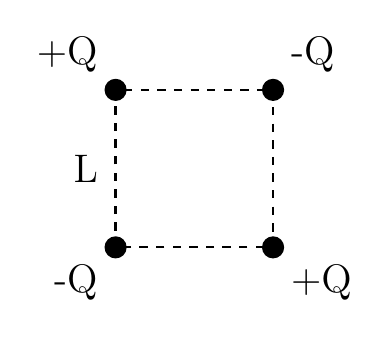
\begin{tikzpicture}[
            scale=0.5,
            charge/.style={
                circle, 
                fill=black, 
                inner sep=0pt, 
                minimum size=8pt
            }
        ]
        \draw[dashed, thick] (0,0) rectangle (4,4);
        \node[left, xshift=-0.1cm] at (0,2) {\Large L};
        \node[charge, label=below left:{\Large -Q}] at (0,0) {};
        \node[charge, label=below right:{\Large +Q}] at (4,0) {};
        \node[charge, label=above right:{\Large -Q}] at (4,4) {};
        \node[charge, label=above left:{\Large +Q}] at (0,4) {};
        \end{tikzpicture}
    \end{center}
\end{snippetexercise}

\begin{snippetsolution}{charges-square-force-ex-sol}{Force Between Charges on a Square}
    Due to the symmetry of the system, the magnitude of the force is identical on any charge. We choose to analyze the \(-Q\) charge in the top right. This charge experiences three forces due to the other three charges.
    The two adjacent \(+Q\) charges (at distance \(L\)) exert attractive forces directed along the sides of the square towards them. The magnitude of each of these forces is:
    \[F_{side} = k \frac{Q^2}{L^2}\]
    The opposite \(-Q\) charge (at the diagonal distance \(L\sqrt{2}\)) exerts a repulsive force along the diagonal, outwards. The magnitude of this force is:
    \[F_{diag} = k \frac{Q^2}{(L\sqrt{2})^2} = k \frac{Q^2}{2L^2}\]
    The two attractive forces \(F_{side}\) are orthogonal to each other. Their resultant points towards the center of the square, along the diagonal, and is equal to:
    \[F_{attr\_tot} = \sqrt{F_{side}^2 + F_{side}^2} = F_{side}\sqrt{2} = k \frac{Q^2}{L^2}\sqrt{2}\]
    The repulsive force \(F_{diag}\) lies on the same diagonal but points in the opposite direction (outwards). The total net force is the difference between their magnitudes:
    \[F_{net} = F_{attr\_tot} - F_{diag} = k \frac{Q^2}{L^2}\left(\sqrt{2} - \frac{1}{2}\right)\]
    Let's convert the data into the SI: \(Q = 20 \times 10^{-6} \mathrm{C}\), \(L = 0.6 \mathrm{m}\) and we use \(k \approx 8.99 \times 10^9 \mathrm{N \cdot m^2/C^2}\):
    \[k \frac{Q^2}{L^2} = 8.99 \times 10^9 \frac{(20 \times 10^{-6})^2}{0.6^2} \approx 9.99 \mathrm{N} \approx 10.0 \mathrm{N}\]
    Substituting this value:
    \[F_{net} = 10.0 \cdot (1.414 - 0.5) = 10.0 \cdot 0.914 = 9.14 \mathrm{N}\]
    The magnitude of the electrostatic force on any of the charges is \(9.14 \mathrm{N}\) directed towards the center of the square.
\end{snippetsolution}

\begin{snippetexercise}{lorentz-force-particles-ex}{Lorentz Force on Charged Particles}
    A magnetic field is directed out of the screen.
    Two charged particles enter from the top and follow the paths shown in the figure.
    Which of the following statements is correct?
    \begin{center}
        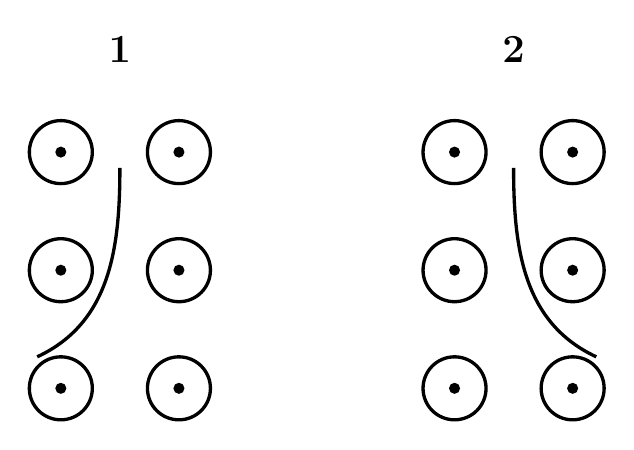
\begin{tikzpicture}[
            B-field/.style={
                very thick,
                circle,
                minimum size=0.8cm, 
                draw,
                append after command={
                    \pgfextra{
                        \fill (\tikzlastnode.center) circle (2pt); 
                    }
                }
            }
        ]
        \node at (0.75, 4.3) {\Large \textbf{1}};
        \foreach \row in {0, 1, 2} {
            \foreach \col in {0, 1} {
                \node[B-field] at (\col * 1.5, \row * 1.5) {};
            }
        }
        \draw[very thick] (-0.3, 0.4) to[out=25, in=-90] (0.75, 2.8);
        \begin{scope}[xshift=5cm]
            \node at (0.75, 4.3) {\Large \textbf{2}};
            \foreach \row in {0, 1, 2} {
                \foreach \col in {0, 1} {
                    \node[B-field] at (\col * 1.5, \row * 1.5) {};
                }
            }
            \draw[very thick] (1.8, 0.4) to[out=155, in=-90] (0.75, 2.8);
        \end{scope}
        \end{tikzpicture}
    \end{center}
    \begin{enumerate}[label=\Alph*]
        \item Particle 1 has a positive charge and particle 2 has a negative charge;
        \item Particle 2 has a positive charge and particle 1 has a negative charge;
        \item Both particles have a positive charge;
        \item Both particles have a negative charge;
        \item The direction of the paths depends on the magnitude of the velocity and not on the sign of the charge.
    \end{enumerate}
\end{snippetexercise}

\begin{snippetsolution}{lorentz-force-particles-ex-sol}{Lorentz Force on Charged Particles}
    Particle 1 has a positive charge and particle 2 has a negative charge
    because \(\vec{F} = q\vec{v} \times \vec{B}\).
\end{snippetsolution}

\begin{snippetexercise}{electromagnetic-induction-coil-ex}{Electromagnetic Induction}
    A coil consisting of \(N=4\) turns has an area of \(A=200~\mathrm{cm}^{2}\) (\(0.02~\mathrm{m}^2\)). It is placed in a uniform magnetic field perpendicular to the surface. The field varies from \(25~\mathrm{mT}\) to \(10~\mathrm{mT}\) in a time interval \(\Delta t=5~\mathrm{s}\). Given that the resistance of the coil is \(R=5.0~\Omega\), calculate the induced current intensity.
\end{snippetexercise}

\begin{snippetsolution}{electromagnetic-induction-coil-ex-sol}{Electromagnetic Induction}
    We apply the Faraday-Lenz law combined with Ohm's law:
    \[
    I = \frac{\text{emf}}{R} = \frac{1}{R} \cdot N \cdot \frac{\Delta\Phi}{\Delta t}
    \]
    Considering the variation of the field \(\Delta B = 15 \cdot 10^{-3}~\mathrm{T}\):
    \[
    I = \frac{4 \cdot 0.02 \cdot 15 \cdot 10^{-3}}{5 \cdot 5} = 0.000048~\mathrm{A} = 48~\mathrm{mA}
    \]
\end{snippetsolution}

\begin{snippetexercise}{lorentz-force-direction-ex}{Direction of the Lorentz Force}
    A positive charge moves with velocity along the positive x-axis in the presence of a magnetic field \(B\) directed along the positive z-axis. Determine the direction of the force acting on the charge.
\end{snippetexercise}

\begin{snippetsolution}{lorentz-force-direction-ex-sol}{Direction of the Lorentz Force}
    Using the right-hand rule for the cross product \(\vec{F} = q\vec{v} \times \vec{B}\):
    \begin{itemize}
        \item Velocity vector \(\vec{v}\) towards \(+x\).
        \item Field vector \(\vec{B}\) towards \(+z\).
        \item The resulting force \(\vec{F}\) is directed along the negative \(y\) axis.
    \end{itemize}
\end{snippetsolution}

\begin{snippetexercise}{electrostatic-force-superposition-ex}{Superposition of Electrostatic Forces}
    Three charges are arranged on a line: \(Q=30\cdot10^{-6}~\mathrm{C}\), \(q=5\cdot10^{-6}~\mathrm{C}\), and a charge \(-2Q\) (from calculation). The charge \(q\) is placed centrally at a distance \(d=0.30~\mathrm{m}\) from the other two. Calculate the total force acting on \(q\).
\end{snippetexercise}

\begin{snippetsolution}{electrostatic-force-superposition-ex-sol}{Superposition of Electrostatic Forces}
    The total force is the vector sum of the forces exerted by \(Q\) and \(-2Q\):
    \[
    F_{tot} = \frac{1}{4\pi\epsilon_{0}}\cdot\frac{q\cdot Q}{d^{2}} + \frac{1}{4\pi\epsilon_{0}}\cdot\frac{q\cdot 2Q}{d^{2}}
    \]
    Inserting the values (with \(k=9\cdot10^{9}~\mathrm{Nm^{2}/C^{2}}\)):
    \[
    F_{tot} = 9\cdot10^{9} \cdot 5\cdot10^{-6} \cdot \left(\frac{30\cdot10^{-6}}{0.09} + \frac{60\cdot10^{-6}}{0.09}\right) = 7.5~\mathrm{N}
    \]
\end{snippetsolution}

\begin{snippetexercise}{inductor-energy-ex}{Energy of an Inductor}
    Calculate the energy stored in an inductor with inductance \(L=0.5\cdot10^{-3}~\mathrm{H}\) when a current \(i=4.0~\mathrm{A}\) flows through it.
\end{snippetexercise}

\begin{snippetsolution}{inductor-energy-ex-sol}{Energy of an Inductor}
    The energy \(U\) is given by the formula:
    \[
    U = \frac{1}{2}Li^{2} = 0.5 \cdot 0.5\cdot10^{-3} \cdot 4^{2} = 4\cdot10^{-3}~\mathrm{J} \quad (4~\mathrm{mJ})
    \]
\end{snippetsolution}

\begin{snippetexercise}{capacitors-series-ex}{Capacitors in Series}
    Two capacitors \(C_{1}=15~\mu\mathrm{F}\) and \(C_{2}=30~\mu\mathrm{F}\) are connected in series to a source of \(\Delta V=50~\mathrm{V}\). Calculate the charge on \(C_{2}\).
\end{snippetexercise}

\begin{snippetsolution}{capacitors-series-ex-sol}{Capacitors in Series}
    In series, the charge \(q\) is identical on both capacitors and equal to the charge of the equivalent capacitance:
    \[
    1/C_{eq} = 1/15 + 1/30 \Rightarrow C_{eq} = 10~\mu\mathrm{F}
    \]
    \[
    q = C_{eq} \cdot \Delta V = 10\cdot10^{-6} \cdot 50 = 5\cdot10^{-4}~\mathrm{C}
    \]
\end{snippetsolution}

\begin{snippetexercise}{electric-field-flux-gauss-ex}{Electric Field Flux (Gauss's Law)}
    A sphere has a surface charge density \(\sigma=4.0~\mathrm{nC/m^{2}}\) and radius \(r=0.02~\mathrm{m}\). Calculate the electric flux through a spherical Gaussian surface of radius \(0.04~\mathrm{m}\).
\end{snippetexercise}

\begin{snippetsolution}{electric-field-flux-gauss-ex-sol}{Electric Field Flux (Gauss's Law)}
    The flux depends only on the total enclosed charge:
    \[
    Q_{tot} = \sigma \cdot 4\pi r^{2} = 4\cdot10^{-9} \cdot 4\pi \cdot (0.02)^{2}
    \]
    \[
    \Phi = Q_{tot}/\epsilon_{0} \approx 2.27~\mathrm{Vm}
    \]
\end{snippetsolution}

\begin{snippetexercise}{em-waves-parameters-ex}{Electromagnetic Wave Parameters}
    Given a solar radiation intensity \(I=1340~\mathrm{W/m}^{2}\), determine the amplitude of the electric field \(E_{0}\) and the magnetic field \(B_{0}\).
\end{snippetexercise}

\begin{snippetsolution}{em-waves-parameters-ex-sol}{Electromagnetic Wave Parameters}
    \[
    E_{0} = \sqrt{2I/(c\epsilon_{0})} \approx 1000~\mathrm{V/m}
    \]
    \[
    B_{0} = E_{0}/c \approx 3.33\cdot10^{-6}~\mathrm{T}
    \]
\end{snippetsolution}

\begin{snippetexercise}{magnetic-field-infinite-wires-ex}{Magnetic Field of Infinite Wires}
    Two parallel wires separated by a distance \(d=5~\mathrm{mm}\) carry opposite currents \(i=60~\mathrm{A}\). Calculate the magnetic field \(B\) at an internal point located at \(r_{1}=2~\mathrm{mm}\) from the first wire.
\end{snippetexercise}

\begin{snippetsolution}{magnetic-field-infinite-wires-ex-sol}{Magnetic Field of Infinite Wires}
    Since the currents are opposite, the fields between the wires sum up. With \(r_{1}=0.002~\mathrm{m}\) and \(r_{2}=0.003~\mathrm{m}\):
    \[
    B_{tot} = \frac{\mu_{0} \cdot i}{2\pi} \cdot \left(\frac{1}{r_{1}} + \frac{1}{r_{2}}\right)
    \]
    \[
    B_{tot} = 2\cdot10^{-7} \cdot 60 \cdot (500 + 333.3) \approx 2\cdot10^{-2}~\mathrm{T} \quad (20~\mathrm{mT})
    \]
\end{snippetsolution}

\begin{snippetexercise}{electrostatic-potential-difference-ex}{Electrostatic Potential Difference}
    Calculate the potential difference between two points A and B generated by a system of two point charges \(q\) and \(Q\).
\end{snippetexercise}

\begin{snippetsolution}{electrostatic-potential-difference-ex-sol}{Electrostatic Potential Difference}
    Calculate the potential at each point as the sum of the potentials of the individual charges (\(V=k\sum q_{i}/r_{i}\)). Following the numerical steps from the sheet:
    \[
    V_{A} - V_{B} = +60~\mathrm{V}
    \]
\end{snippetsolution}

\begin{snippetexercise}{resistance-series-circuit-ex}{Resistance in a Series Circuit}
    A circuit is powered by an \(\text{emf}=20~\mathrm{V}\). When two resistors \(R_{1}\) and \(R_{2}\) are in series, a current \(i=1.0~\mathrm{A}\) flows. Knowing that \(R_{2}=15~\Omega\), determine \(R_{1}\).
\end{snippetexercise}

\begin{snippetsolution}{resistance-series-circuit-ex-sol}{Resistance in a Series Circuit}
    From Ohm's law for the series circuit:
    \[
    R_{tot} = R_{1} + R_{2} = \frac{V}{i}
    \]
    \[
    R_{1} + 15 = \frac{20}{1.0} = 20~\Omega
    \]
    \[
    R_{1} = 20 - 15 = 5~\Omega
    \]
\end{snippetsolution}

\begin{snippetexercise}{capacitor-circuit-ex}{Capacitor Circuit}
    Given a circuit powered by a voltage \(V_{0}=18~\mathrm{V}\) composed of three capacitors \(C_{1}=20\mu \mathrm{F}\), \(C_{2}=10\mu \mathrm{F}\), and \(C_{3}=30\mu \mathrm{F}\), determine the equivalent capacitance and the charge \(q_{1}\) on the first capacitor.
\end{snippetexercise}

\begin{snippetsolution}{capacitor-circuit-ex-sol}{Capacitor Circuit}
    \textbf{Capacitance in parallel:} \(C_{2}\) and \(C_{3}\) are in parallel:
    \[
    C_{23} = C_{2} + C_{3} = 10\mu \mathrm{F} + 30\mu \mathrm{F} = 40\mu \mathrm{F}
    \]
    \textbf{Equivalent capacitance:} \(C_{1}\) is in series with \(C_{23}\):
    \[
    \frac{1}{C_{eq}} = \frac{1}{C_{1}} + \frac{1}{C_{23}} = \frac{1}{20} + \frac{1}{40} = \frac{3}{40}\mu \mathrm{F}^{-1}
    \]
    \[
    \Rightarrow C_{eq} = \frac{40}{3}\mu \mathrm{F} \approx 13.33~\mu \mathrm{F}
    \]
    
    \textbf{Charge \(q_{1}\):} In a series circuit, the charge on each component is equal to the total charge supplied by the source:
    \[
    q_{1} = q_{tot} = C_{eq} \cdot V_{0} = \frac{40}{3} \cdot 18 = 240~\mu \mathrm{C}
    \]
\end{snippetsolution}

\begin{snippetexercise}{charged-particle-acceleration-ex}{Charged Particle Acceleration}
    A proton (\(m_{p}=1.67\cdot10^{-27}\) kg, \(q=1.6\cdot10^{-19}\mathrm{C}\)) starts from rest and is accelerated by a potential difference \(\Delta V=4\cdot10^{3}\) V. Calculate the final velocity \(v\).
\end{snippetexercise}

\begin{snippetsolution}{charged-particle-acceleration-ex-sol}{Charged Particle Acceleration}
    Applying the principle of conservation of energy (\(K=W\)):
    \[
    \frac{1}{2}m_{p}v^{2} = q\Delta V \Rightarrow v = \sqrt{\frac{2q\Delta V}{m_{p}}}
    \]
    \[
    v = \sqrt{\frac{2\cdot1.6\cdot10^{-19}\cdot4000}{1.67\cdot10^{-27}}} \approx 8.76\cdot10^{5}~\mathrm{m/s}
    \]
\end{snippetsolution}

\begin{snippetexercise}{em-waves-amplitude-ex}{Electromagnetic Waves}
    In a plane electromagnetic wave in a vacuum, the maximum electric field is \(E_{max}=600~\mathrm{V/m}\). Calculate the amplitude of the magnetic field \(B_{max}\).
\end{snippetexercise}

\begin{snippetsolution}{em-waves-amplitude-ex-sol}{Electromagnetic Waves}
    From the fundamental relationship between the field magnitudes in a plane wave (\(E=cB\)):
    \[
    B_{max} = \frac{E_{max}}{c} = \frac{600}{3\cdot10^{8}} = 2\cdot10^{-6}~\mathrm{T} \quad (\text{i.e. } 2~\mu \mathrm{T})
    \]
\end{snippetsolution}

\begin{snippetexercise}{point-charges-force-ex}{Force Between Point Charges}
    Three charges are aligned on the x-axis: \(q_{1}=40\mu \mathrm{C}\) at \(x_{1}=-20\) cm, \(q_{2}=50\mu \mathrm{C}\) at \(x_{2}=30\) cm, and \(q_{3}=4\mu \mathrm{C}\) at the origin (\(x=0\)). Calculate the resultant force on \(q_{3}\).
\end{snippetexercise}

\begin{snippetsolution}{point-charges-force-ex-sol}{Force Between Point Charges}
    Assuming all charges are positive, \(q_{3}\) experiences a push to the right from \(q_{1}\) (\(F_{13}\)) and a push to the left from \(q_{2}\) (\(F_{23}\)):
    \[
    F_{tot} = |F_{13}| - |F_{23}| = \frac{q_{3}}{4\pi\epsilon_{0}}\left(\frac{q_{1}}{r_{1}^{2}} - \frac{q_{2}}{r_{2}^{2}}\right)
    \]
    \[
    F_{tot} = (9\cdot10^{9})\cdot(4\cdot10^{-6})\cdot\left(\frac{40\cdot10^{-6}}{0.2^{2}} - \frac{50\cdot10^{-6}}{0.3^{2}}\right) \approx 16~\mathrm{N} \quad (\text{direction } +x)
    \]
\end{snippetsolution}

\begin{snippetexercise}{faraday-lenz-law-loop-ex}{Faraday-Lenz Law}
    A circular loop is immersed in a uniform magnetic field \(B=1.5~\mathrm{T}\) perpendicular to the plane of the loop. The radius of the loop increases linearly with time according to the law \(r(t) = r_{0}+vt\) with \(r_{0}=0.12~\mathrm{m}\) and \(v=0.03~\mathrm{m/s}\). Calculate the instantaneous induced emf.
\end{snippetexercise}

\begin{snippetsolution}{faraday-lenz-law-loop-ex-sol}{Faraday-Lenz Law}
    The magnetic flux is \(\Phi(B) = B \cdot A = B \cdot \pi r^{2}\).
    \[
    E = -\frac{d\Phi}{dt} = -B\pi\frac{d}{dt}(r^{2}) = -B\pi\left(2r\cdot\frac{dr}{dt}\right)
    \]
    Substituting the values at the initial instant:
    \[
    E = -1.5 \cdot \pi \cdot 2 \cdot 0.12 \cdot 0.03 \approx -33.9~\mathrm{mV}
    \]
\end{snippetsolution}

\begin{snippetexercise}{joule-effect-ex}{Joule Effect}
    Calculate the thermal energy dissipated in a time \(\Delta t=120\) s by a resistor \(R=150~\Omega\) connected to a voltage \(\Delta V=20~\mathrm{V}\).
\end{snippetexercise}

\begin{snippetsolution}{joule-effect-ex-sol}{Joule Effect}
    \[
    E = P \cdot \Delta t = \frac{\Delta V^{2}}{R} \cdot \Delta t = \frac{20^{2}}{150} \cdot 120 = 320~\mathrm{J}
    \]
\end{snippetsolution}

\begin{snippetexercise}{rlc-circuit-sinusoidal-ex}{RLC Circuit in Sinusoidal Regime}
    A series RLC circuit has \(R=100~\Omega\), \(L=1~\mathrm{H}\), \(C=2\mu \mathrm{F}\). The source supplies \(V(t) = 100 \sin(500t)\). Calculate the effective current \(I_{eff}\).
\end{snippetexercise}

\begin{snippetsolution}{rlc-circuit-sinusoidal-ex-sol}{RLC Circuit in Sinusoidal Regime}
    \begin{enumerate}
        \item \textbf{Angular frequency:} \(\omega = 500~\mathrm{rad/s}\)
        \item \textbf{Reactances:}
        \[
        X_{L} = \omega L = 500 \cdot 1 = 500~\Omega
        \]
        \[
        X_{C} = \frac{1}{\omega C} = \frac{1}{500 \cdot 2 \cdot 10^{-6}} = 1000~\Omega
        \]
        \item \textbf{Impedance:}
        \[
        Z = \sqrt{R^{2} + (X_{L} - X_{C})^{2}} = \sqrt{100^{2} + (500 - 1000)^{2}} \approx 509.9~\Omega
        \]
        \item \textbf{Effective current:}
        \[
        V_{eff} = \frac{V_{max}}{\sqrt{2}} = \frac{100}{\sqrt{2}} \approx 70.71~\mathrm{V}
        \]
        \[
        I_{eff} = \frac{V_{eff}}{Z} = \frac{70.71}{509.9} \approx 0.139~\mathrm{A}
        \]
    \end{enumerate}
\end{snippetsolution}

\begin{snippetexercise}{wire-resistance-calculation-ex}{}
    Calculate the resistance in \(\Omega\) of a wire with resistivity \(3.2 \cdot 10^{-8}\)
    \(\Omega \text{m}\), with length \(2.5\) meters and diameter \(0.5 \text{mm}\).
\end{snippetexercise}

\begin{snippetsolution}{wire-resistance-calculation-ex-sol}{}
    We use the second law of Ohm: \(R = \rho \frac{L}{A}\). \\
    Convert diameter to radius and to meters: \(r = \frac{d}{2} = 0.25 \, \text{mm} = 2.5 \cdot 10^{-4} \, \text{m}\). \\
    The cross-sectional area is \(A = \pi r^2 = \pi (2.5 \cdot 10^{-4})^2 \approx 1.96 \cdot 10^{-7} \, \text{m}^2\). \\
    Calculation:
    \[
    R = (3.2 \cdot 10^{-8}) \frac{2.5}{1.96 \cdot 10^{-7}} \approx \frac{8 \cdot 10^{-8}}{1.96 \cdot 10^{-7}} \approx 0.408 \, \Omega
    \]
\end{snippetsolution}

\begin{snippetexercise}{em-wave-B-max-ex}{}
    If the maximum value of the \(E\) component of an electromagnetic wave is \(600 \text{V/m}\), what is the maximum of the \(B\) component?
\end{snippetexercise}

\begin{snippetsolution}{em-wave-B-max-ex-sol}{}
    In an electromagnetic wave in a vacuum, the relationship between the field amplitudes is \(E = cB\), where \(c \approx 3 \cdot 10^8 \, \text{m/s}\).
    \[
    B = \frac{E}{c} = \frac{600}{3 \cdot 10^8} = 200 \cdot 10^{-8} = 2.0 \cdot 10^{-6} \, \text{T} = 2.0 \, \mu\text{T}
    \]
\end{snippetsolution}

\begin{snippetexercise}{square-charges-electric-field-ex}{}
    Two charges are placed on a square of side \(1.5\) meters, one of \(2 \text{nC}\)
    and one of \(3 \text{nC}\) on two opposite vertices. What is the intensity of the electric
    field on one of the other two vertices?
\end{snippetexercise}

\begin{snippetsolution}{square-charges-electric-field-ex-sol}{}
    Let the charges be \(q_1 = 2\,\text{nC}\) and \(q_2 = 3\,\text{nC}\). The vertex considered is adjacent to both, so the distance from each charge is \(r = 1.5\,\text{m}\). The generated electric fields are perpendicular to each other.
    \[ E_1 = k \frac{q_1}{r^2} = (8.99 \cdot 10^9) \frac{2 \cdot 10^{-9}}{1.5^2} \approx 8.0 \, \text{N/C} \]
    \[ E_2 = k \frac{q_2}{r^2} = (8.99 \cdot 10^9) \frac{3 \cdot 10^{-9}}{1.5^2} \approx 12.0 \, \text{N/C} \]
    The total field is the vector sum (Pythagoras):
    \[ E_{tot} = \sqrt{E_1^2 + E_2^2} = \sqrt{8^2 + 12^2} = \sqrt{64 + 144} \approx 14.4 \, \text{N/C} \]
\end{snippetsolution}

\begin{snippetexercise}{charged-sphere-electric-field-ex}{}
    A sphere of volume \(12 \text{cm}^3\) is filled with a non-conducting material
    with a uniformly distributed charge of \(30 \text{pC}\) throughout the volume.
    What is the electric field intensity at \(1.0 \text{cm}\) from the center?
\end{snippetexercise}

\begin{snippetsolution}{charged-sphere-electric-field-ex-sol}{}
    Let's find the radius of the sphere \(R\). \(V = \frac{4}{3}\pi R^3 \Rightarrow R = \sqrt[3]{\frac{3V}{4\pi}}\).
    With \(V=12\), \(R \approx 1.42\,\text{cm}\). Since the requested distance \(r=1.0\,\text{cm}\) is less than \(R\), we are inside the distribution.
    The internal field of a uniformly charged insulating sphere is:
    \[ E = \frac{Q_{tot} r}{4\pi \epsilon_0 R^3} = \frac{\rho r}{3\epsilon_0} \]
    More simply, using the proportion of enclosed charge \(Q_{enc} = Q_{tot} \frac{r^3}{R^3}\):
    \[ E = k \frac{Q_{enc}}{r^2} = k \frac{Q_{tot} r}{R^3} \]
    \[ E = (8.99 \cdot 10^9) \frac{30 \cdot 10^{-12} \cdot 0.01}{(0.0142)^3} \approx 941 \, \text{N/C} \]
\end{snippetsolution}

\begin{snippetexercise}{rectangular-loop-fem-ex}{}
    Consider a rectangular loop of \(0.2 \text{m}\) with a uniform magnetic field perpendicular
    to the plane of the loop. The magnetic field intensity is \(B = 0.4 T \cdot e^{t/J}\) seconds and
    \(J = 4.0\). Calculate induced emf at \(t = 2.0\) seconds.
\end{snippetexercise}

\begin{snippetsolution}{rectangular-loop-fem-ex-sol}{}
    Assume the loop is square with side \(l=0.2\,\text{m}\), so Area \(A = 0.04\,\text{m}^2\).
    Faraday-Neumann-Lenz Law: \(\mathcal{E} = - \frac{d\Phi_B}{dt} = -A \frac{dB}{dt}\).
    Given \(B(t) = 0.4 e^{t/4}\), the derivative is \(\frac{dB}{dt} = 0.4 \cdot \frac{1}{4} e^{t/4} = 0.1 e^{t/4}\).
    At \(t=2.0\): \(\frac{dB}{dt} = 0.1 e^{0.5} \approx 0.165 \, \text{T/s}\).
    \[ |\mathcal{E}| = 0.04 \cdot 0.165 \approx 0.0066 \, \text{V} = 6.6 \, \text{mV} \]
\end{snippetsolution}

\begin{snippetexercise}{wire-force-parallel-field-ex}{}
    Consider a \(2\) meter cable suspended parallel to a uniform magnetic field of \(0.5 T\),
    carried by a current of \(0.6 A\). Find the force in Newtons applied to the cable.
\end{snippetexercise}

\begin{snippetsolution}{wire-force-parallel-field-ex-sol}{}
    The force on a current-carrying wire is \(F = I L B \sin(\theta)\).
    The text specifies that the cable is \textbf{parallel} to the magnetic field, so \(\theta = 0^\circ\) (or \(180^\circ\)).
    Since \(\sin(0) = 0\), the magnetic force is:
    \[ F = 0 \, \text{N} \]
\end{snippetsolution}

\begin{snippetexercise}{resistor-potential-difference-electrons-ex}{}
    If \(5 \times 10^{21}\) electrons enter a \(20 \Omega\) resistor in \(10 \text{min}\), what is the potential
    difference in \(V\) across the resistor?
\end{snippetexercise}

\begin{snippetsolution}{resistor-potential-difference-electrons-ex-sol}{}
    Let's calculate the total charge first and then the current.
    \(Q = N \cdot e = 5 \cdot 10^{21} \cdot 1.6 \cdot 10^{-19} = 800 \, \text{C}\).
    The time in seconds is \(t = 10 \cdot 60 = 600 \, \text{s}\).
    Current \(I = \frac{Q}{t} = \frac{800}{600} = \frac{4}{3} \, \text{A} \approx 1.33 \, \text{A}\).
    Ohm's Law:
    \[ V = R \cdot I = 20 \cdot \frac{4}{3} = \frac{80}{3} \approx 26.7 \, \text{V} \]
\end{snippetsolution}

\begin{snippetexercise}{capacitors-parallel-energy-ex}{Energy of Capacitors in Parallel}
    A \(15 \mu\mathrm{F}\) capacitor and a \(25 \mu\mathrm{F}\) capacitor
    are connected in parallel, and a potential difference of 60 Volts is applied to this combination.
    How much energy is stored in this combination of capacitors?
\end{snippetexercise}

\begin{snippetsolution}{capacitors-parallel-energy-ex-sol}{Energy of Capacitors in Parallel}
    For two capacitors connected in parallel, the equivalent capacitance \(C_{eq}\) is given by the sum of the individual capacitances:
    \[ C_{eq} = C_1 + C_2 = 15 \mu\mathrm{F} + 25 \mu\mathrm{F} = 40 \mu\mathrm{F} = 40 \times 10^{-6} \mathrm{F} \]
    The electric potential energy \(U\) stored in a capacitor (or a system of capacitors) can be calculated using the formula:
    \[ U = \frac{1}{2} C_{eq} V^2 \]
    Substituting the values provided by the problem:
    \[ U = \frac{1}{2} (40 \times 10^{-6} \mathrm{F}) (60 \mathrm{V})^2 = 20 \times 10^{-6} \cdot 3600 = 0.072 \mathrm{J} \]
    The energy stored in the combination of capacitors is equal to \(0.072 \mathrm{J}\) (i.e., \(72 \mathrm{mJ}\)).
\end{snippetsolution}

\begin{snippetexercise}{em-wave-intensity-ex}{Intensity of Electromagnetic Waves}
    A radio station emits EM waves in all directions from an antenna on top of a mountain with
    a power of \(100 \mathrm{kW}\). Determine the intensity 
    \(S\) (in \(\mathrm{W/m}^2\)) of the signal at a distance of \(10 \mathrm{km}\).
\end{snippetexercise}

\begin{snippetsolution}{em-wave-intensity-ex-sol}{Intensity of Electromagnetic Waves}
    The antenna emits electromagnetic waves isotropically (in all directions). Therefore, the power \(P\) is distributed uniformly over increasing spherical surfaces with area \(A = 4\pi r^2\).
    The intensity \(S\) of the wave at a distance \(r\) is calculated as:
    \[ S = \frac{P}{A} = \frac{P}{4\pi r^2} \]
    Let's convert the data into the International System:
    \(P = 100 \mathrm{kW} = 100 \times 10^3 \mathrm{W}\)
    \(r = 10 \mathrm{km} = 10 \times 10^3 \mathrm{m}\)
    Substitute the values into the equation:
    \[ S = \frac{100 \times 10^3 \mathrm{W}}{4\pi (10 \times 10^3 \mathrm{m})^2} = \frac{10^5}{4\pi \cdot 10^8} = \frac{1}{4000\pi} \approx 7.96 \times 10^{-5} \mathrm{W/m}^2 \]
    The signal intensity at a distance of \(10 \mathrm{km}\) is approximately \(7.96 \times 10^{-5} \mathrm{W/m}^2\).
\end{snippetsolution}

\begin{snippetexercise}{ampere-law-inside-wire-ex}{Magnetic Field Inside a Wire}
    A straight wire with a diameter of \(2.0 \mathrm{mm}\) carries a current of
    \(25 \mathrm{A}\). What is the magnitude of the magnetic field at \(0.50 \mathrm{mm}\) from the axis of the wire?
\end{snippetexercise}

\begin{snippetsolution}{ampere-law-inside-wire-ex-sol}{Magnetic Field Inside a Wire}
    The diameter of the wire is \(D = 2.0 \mathrm{mm}\), so its radius is \(R = 1.0 \mathrm{mm}\).
    Since the magnitude of the field is requested at a distance \(r = 0.50 \mathrm{mm}\) from the axis, we are \textit{inside} the wire (\(r < R\)).
    Assuming a uniform current density across the wire's cross-section, Ampère's law provides the magnitude of the internal magnetic field:
    \[ B = \frac{\mu_0 I r}{2\pi R^2} \]
    Knowing that the magnetic permeability in a vacuum is \(\mu_0 = 4\pi \times 10^{-7} \mathrm{T \cdot m/A}\), we substitute the values (making sure to convert them to meters):
    \[ B = \frac{(4\pi \times 10^{-7} \mathrm{T \cdot m/A}) (25 \mathrm{A}) (0.50 \times 10^{-3} \mathrm{m})}{2\pi (1.0 \times 10^{-3} \mathrm{m})^2} \]
    \[ B = \frac{2 \times 10^{-7} \cdot 12.5 \times 10^{-3}}{10^{-6}} = 25 \times 10^{-4} \mathrm{T} = 2.5 \mathrm{mT} \]
    The magnitude of the magnetic field at \(0.50 \mathrm{mm}\) from the axis is \(2.5 \times 10^{-3} \mathrm{T}\) (or \(2.5 \mathrm{mT}\)).
\end{snippetsolution}

\begin{snippetexercise}{electric-field-parallel-planes-ex}{Electric Field of Parallel Planes}
    A uniform charge density \((8.0 \mathrm{nC/m^2})\)
    is distributed over the entire \(xy\) plane.
    A uniform charge density \((5.0 \mathrm{nC/m^2})\)
    is distributed on a parallel plane defined by \(z = 2.0 \mathrm{m}\).
    Determine the magnitude of the electric field for any point
    with \(z = 1.0 \mathrm{m}\).
\end{snippetexercise}

\begin{snippetsolution}{electric-field-parallel-planes-ex-sol}{Electric Field of Parallel Planes}
    The electric field generated by an infinite plane with surface charge density \(\sigma\) is uniform and has a magnitude:
    \[ E = \frac{|\sigma|}{2\varepsilon_0} \]
    where \(\varepsilon_0 \approx 8.854 \times 10^{-12} \mathrm{C^2/(N \cdot m^2)}\). Since both distributions have a positive sign, the electric field vectors will point outward from each plane.
    The point in question is located at \(z = 1.0 \mathrm{m}\), which is \textit{between} the two planes (located at \(z = 0\) and \(z = 2.0 \mathrm{m}\)). 
    In this region:
    \begin{itemize}
        \item Plane 1 (\(z = 0\)) with \(\sigma_1 = 8.0 \mathrm{nC/m^2}\) pushes upwards (positive direction of the \(z\) axis). 
        \item Plane 2 (\(z = 2.0\)) with \(\sigma_2 = 5.0 \mathrm{nC/m^2}\) pushes downwards (negative direction of the \(z\) axis).
    \end{itemize}
    The two fields have the same direction and opposite signs. The total magnitude, by the superposition principle, is given by the difference of their magnitudes:
    \[ E_{tot} = |E_1 - E_2| = \left| \frac{\sigma_1}{2\varepsilon_0} - \frac{\sigma_2}{2\varepsilon_0} \right| = \frac{\sigma_1 - \sigma_2}{2\varepsilon_0} \]
    Substituting the values:
    \[ E_{tot} = \frac{(8.0 - 5.0) \times 10^{-9} \mathrm{C/m^2}}{2 \cdot 8.854 \times 10^{-12} \mathrm{C^2/(N \cdot m^2)}} = \frac{3.0 \times 10^{-9}}{17.708 \times 10^{-12}} \approx 169.4 \mathrm{V/m} \]
    The magnitude of the electric field at any point with \(z = 1.0 \mathrm{m}\) is approximately \(169.4 \mathrm{V/m}\) (directed upwards).
\end{snippetsolution}

\begin{snippetexercise}{light-bulb-resistance-ex}{Resistance of a Light Bulb}
    A \(100\) Watt light bulb is connected to a \(120\) Volt source.
    What is the resistance of the light bulb in \(\Omega\)?
\end{snippetexercise}

\begin{snippetsolution}{light-bulb-resistance-ex-sol}{Resistance of a Light Bulb}
    The electrical power \(P\) dissipated in a resistor (like the filament of the light bulb) is related to the potential difference \(V\) and its resistance \(R\) by the formula:
    \[ P = \frac{V^2}{R} \]
    To find the resistance, we isolate \(R\) in the equation:
    \[ R = \frac{V^2}{P} \]
    Substituting the values provided by the text (Power \(P = 100 \mathrm{W}\), voltage \(V = 120 \mathrm{V}\)):
    \[ R = \frac{(120 \mathrm{V})^2}{100 \mathrm{W}} = \frac{14400}{100} = 144 \, \Omega \]
    The resistance of the light bulb is \(144 \, \Omega\).
\end{snippetsolution}

\begin{snippetexercise}{faraday-lenz-law-flat-coil-ex}{Faraday-Lenz Law on a Flat Coil}
    A flat coil consisting of \(20\) turns, each with an area of
    \(50 \mathrm{cm^2}\), is positioned perpendicularly to a uniform magnetic field
    whose magnitude increases steadily from \(2.0 \mathrm{T}\) to
    \(6.0 \mathrm{T}\) in \(2.0 \mathrm{s}\).
    If the coil has a total resistance of \(0.40\,\Omega\), what is the magnitude
    of the induced current?
\end{snippetexercise}

\begin{snippetsolution}{faraday-lenz-law-flat-coil-ex-sol}{Faraday-Lenz Law on a Flat Coil}
    According to the Faraday-Neumann-Lenz law, the induced electromotive force \(\mathcal{E}\) in a coil of \(N\) turns is proportional to the variation of the magnetic field flux over time:
    \[\mathcal{E} = N \frac{\Delta \Phi}{\Delta t}\]
    Since the plane of the coil is perpendicular to the magnetic field, the area vector and the magnetic field vector are parallel (\(\cos 0^\circ = 1\)). The variation of the magnetic flux through a single turn depends only on the variation in the magnitude of the field:
    \[\Delta \Phi = A \cdot \Delta B\]
    Let's convert the data into the SI:
    \(N = 20\)
    \(A = 50 \mathrm{cm^2} = 50 \times 10^{-4} \mathrm{m^2} = 5.0 \times 10^{-3} \mathrm{m^2}\)
    \(\Delta B = 6.0 \mathrm{T} - 2.0 \mathrm{T} = 4.0 \mathrm{T}\)
    \(\Delta t = 2.0 \mathrm{s}\)
    We calculate the induced electromotive force:
    \[\mathcal{E} = 20 \cdot \frac{(5.0 \times 10^{-3} \mathrm{m^2})(4.0 \mathrm{T})}{2.0 \mathrm{s}} = 20 \cdot \frac{20.0 \times 10^{-3}}{2.0} = 20 \cdot 10.0 \times 10^{-3} = 0.20 \mathrm{V}\]
    Applying Ohm's law, the magnitude of the induced current \(I\) as a function of the resistance \(R = 0.40 \, \Omega\) is:
    \[I = \frac{\mathcal{E}}{R} = \frac{0.20 \mathrm{V}}{0.40 \, \Omega} = 0.50 \mathrm{A}\]
    The magnitude of the induced current is \(0.50 \mathrm{A}\).
\end{snippetsolution}

\begin{snippetexercise}{electron-acceleration-potential-ex}{Electron Acceleration Potential}
    What potential difference is required to accelerate an electron, initially at rest,
    to a velocity of \(3.0 \times 10^7 \mathrm{m/s}\)?
\end{snippetexercise}

\begin{snippetsolution}{electron-acceleration-potential-ex-sol}{Electron Acceleration Potential}
    By the principle of conservation of energy, the work done by the electric force on an electron is equal to its change in kinetic energy. Since the electron is initially at rest (\(v_i = 0\)), its final kinetic energy is entirely due to the electric potential:
    \[q_e \Delta V = \frac{1}{2} m_e v^2\]
    From which we can isolate the potential difference \(\Delta V\):
    \[\Delta V = \frac{m_e v^2}{2 q_e}\]
    Using the known values for the mass of the electron (\(m_e \approx 9.11 \times 10^{-31} \mathrm{kg}\)) and for its elementary charge (\(q_e \approx 1.60 \times 10^{-19} \mathrm{C}\)), along with the provided velocity (\(v = 3.0 \times 10^7 \mathrm{m/s}\)):
    \[\Delta V = \frac{(9.11 \times 10^{-31} \mathrm{kg})(3.0 \times 10^7 \mathrm{m/s})^2}{2 \cdot 1.60 \times 10^{-19} \mathrm{C}}\]
    \[\Delta V = \frac{9.11 \times 10^{-31} \cdot 9.0 \times 10^{14}}{3.20 \times 10^{-19}} = \frac{81.99 \times 10^{-17}}{3.20 \times 10^{-19}}\]
    \[\Delta V \approx 2562 \mathrm{V} \approx 2.56 \times 10^3 \mathrm{V}\]
    A potential difference of approximately \(2560 \mathrm{V}\) (or \(2.56 \mathrm{kV}\)) is required.
\end{snippetsolution}


\end{document}